\chapter{Introduction and Background}
Redundant, accurate flight vehicle localization has been well-documented over several decades~\cite{zhaoCooperativeLocalizationBased2017,rufaSensorFusionUnmanned2014,tennyRobustNavigationUrban2022,kandemirProbabilisticMeasurementMethod2018}. However, as the threat to GPS signals continues to rise, the need for robust positioning estimation increases. While robust systems already exist to combat incoming interference, these systems are either proprietary or government controlled, making them infeasible for widespread use. Cheaper, robust systems are critical for the safe future of civilian and military flight vehicles. Civilian aircraft feature a wide sensor suite the work in tandem to provide redundancy and safety critical features to maintain safe flight. These aircraft have the space to fit these sensors and the power to run them consistently in all phases of flight (Figure~\ref{fig:weights}), more importantly, the companies that design and build these aircraft also the budget to afford such expensive sensor suites.

\begin{figure}[!ht]\label{fig:weights}
    \centering
    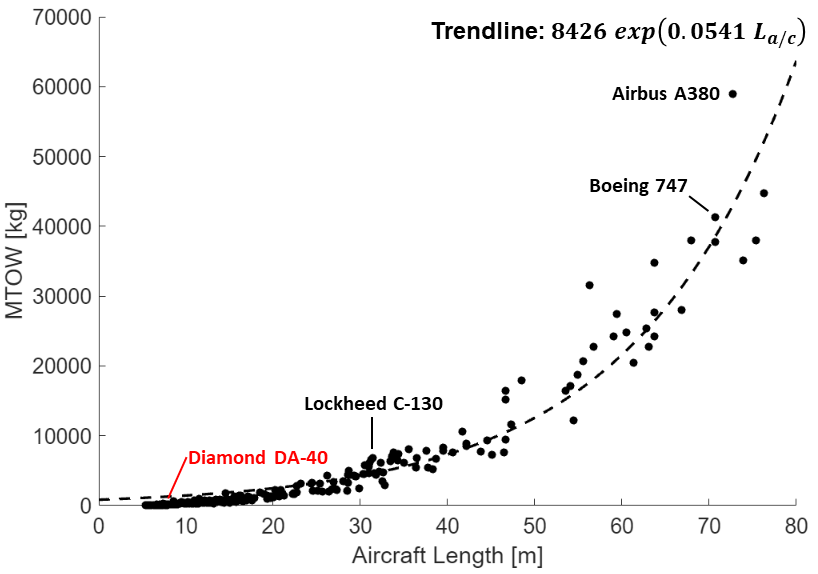
\includegraphics[width=.6\linewidth]{Figures/weights.png}
    \caption{Aircraft with a larger Max Takeoff Operating Weight (MTOW) typically have more space for more complex sensor suites compared to their General Aviation counterparts~\cite{AircraftCharacteristicsDatabase}.}
\end{figure}

Smaller aircraft are not allowed these luxuries, being manufactured with fewer sensors, overall making them less safe. Table~\ref{tbl:sensorsuitecomparison} compares the different sensors onboard a civilian airliner and a civilian general aviation aircraft.

\begin{table}[!ht]\label{tbl:sensorsuitecomparison}
    \caption{Inexhaustive list of sensors available to commercial and general aviation aircraft. (Adapted from~\cite{DiamondAircraftDA40,customerservicesA380AircraftCharacteristics2020})}
    \centering
    \begin{tabular}{lcc}
        \toprule
        \textbf{Sensor}                    & \textbf{Commercial} & \textbf{General Aviation} \\
        \midrule
        Pitot Tubes                        & \(5\)               & \(2\)                     \\
        Distance Measuring Equipment       & \(2\)               & \(1\)                     \\
        Ultra-High Frequency Sensors       & \(2\)               & \(1\)                     \\
        Very-High Frequency Sensors        & \(3\)               & \(2\)                     \\
        Communication Channels             & \(2\)               & \(2\)                     \\
        Outside Air Temperature Sensors    & \(4\)               & \(1\)                     \\
        Fuel Flow Gauge                    & \(4\)               & \(1\)                     \\
        GPS receivers                      & \(2\)               & \(1\)                     \\
        Inertial Measurement Units         & \(3\)               & \(1\)                     \\
        Satellite Communications           & \(1\)               & {--}                      \\
        Specific Impulse Sensors           & \(6\)               & {--}                      \\
        Weather Radar                      & \(1\)               & {--}                      \\
        Traffic Collision Avoidance System & \(4\)               & {--}                      \\
        Radio Altimeter                    & \(3\)               & {--}                      \\

        \bottomrule
    \end{tabular}
\end{table}

Regardless of size, the sensor suite aboard any flight vehicle is able to provide measurements 50 times greater than that of a GPS receiver, so a sensor fusion algorithm is optimal for this situation. Because sensor measurements have inherit errors due to a variety of factors, they can wander or \textit{dead reckon} through time. GPS measurements, although slower, provide measurements that do not drift at cost of being slightly less accurate. Table~\ref{tbl:sensorfusionframeworks} describes the most common sensor fusion frameworks for GPS and INS platforms.
\begin{table}[!ht]\label{tbl:sensorfusionframeworks}
    \caption{Common sensor fusion frameworks used for GPS and INS collection platforms}
    \centering
    \begin{tabular}{clc}
        \toprule
        \textbf{Name}            & \textbf{Level of Measurement}          & \textbf{Typical Error} \\
        \midrule
        \textit{Loosely-Coupled} & GPS Position and Velocity              & \(1~-~3\) [m]          \\
        \textit{Tightly-Coupled} & GPS Pseudorange and Doppler            & \(1~-~2\) [m]          \\
        \textit{Deeply-Coupled}  & GPS Inphase and Quadrature Correlators & \(\leq0.5\) [m]        \\
        \bottomrule
    \end{tabular}
\end{table}
This work presents a deeply-coupled sensor fusion algorithm known as vector tracking. Of the 3 types of GPS and INS sensor fusion frameworks, it is well-documented that deeply coupled provides the most accurate localization between measurement updates~\cite{wattsGPSGLONASSL12019}.
\section{Prior Art}
The objective of this thesis is to investigate the efficacy of position estimation for a flight vehicle in GPS-degraded and GPS-denied conditions. This thesis will analyze the performance through use of a deeply-coupled sensor fusion algorithm utilizing both INS and GPS measurements. The idea of fusing INS measurements and GPS measurements together on a flight vehicle is well-documented. The following subsections scratch the surface of work performed by other authors and their contributions to the field.
\subsection{Sensor Fusion Overview and Variation}
Sensor fusion between GPS and other sensors aboard flight vehicles has existed for years and continues to be developed. A precise, accurate, and robust navigation solution is achievable when redundant, expensive, and high-quality sensor are installed. More information about the sensors found aboard commercial aircraft and smaller aircraft can be found in~\cite{airbuscustomerservicesAirbusA380Aircraft2020} and~\cite{DiamondAircraftDA40}, respectively. Salmon~\cite{salmonExperimentalExplorationLowCost2015} provides an exploratory analysis using ground vehicles and their sensors complimented with a Ground Vehicle Dynamic Model (GVDM) in a tightly-coupled GPS/INS/GVDM sensor fusion. The work of Rhudy~\cite{rhudyDynamicModelaidedSensor2017} is similar to the research presented in this thesis as they present use of known controller inputs into a propriety nonlinear flight vehicle model to perform GPS sensor fusion with low-cost IMUs. Martin~\cite{martinGPSCarrierPhase2017} develops an improved carrier phase tracking approach for precise positioning and vehicle attitude estimation. The vector tracking algorithms described by Martin will be adapted for the GPS and flight vehicle simulation utilized in this thesis.

\subsection{Vehicle Dynamic Model Sensor Fusion}
One of the more common ways to simulate and model a flight vehicle is to use known aerodynamic coefficient tied in with classical flight dynamics to propagate the states in time. The NAVION aircraft model is a nonlinear mathematical aircraft model that uses known aerodynamic coefficient from a single propeller fixed wing Navion aircraft~\cite{nelsonFlightStabilityAutomatic1998}. Rhudy~\cite{rhudyDynamicModelaidedSensor2017} uses the NAVION model included in a Loosely-Coupled sensor fusion with IMU and GPS\@. The paper focuses on using a known aircraft model with incoming piloted control inputs to predict the attitude of the aircraft in time. Khaghani and Skaloud simulate a UAV using initially, known aerodynamic coefficients but feature the coefficients in their Loosely-Coupled sensor fusion algorithm to continuously estimate these variables in their vehicle model. This allows the vehicle dynamic model to change during time as the simulated UAV loses weight due to fuel.Both paper fuse the dynamic model with GPS and IMU measurements at position and velocity level (Loosely-Coupled).~\cite{rhudyDynamicModelaidedSensor2017} uses an Unscented Kalman Filter (UKF) in the navigation filter for \textit{ease of implementation} while Khaghani~\cite{khaghaniAutonomousVehicleDynamic2016,khaghaniAssessmentVDMbasedAutonomous2018} uses a Extended Kalman Filter (EKF) because the 47 state estimation is cumbersome and computationally intensive for the UKF\@. Both Rhudy and Khaghani use simulation environments to perform a monte-carlo analysis. Each IMU is modeled with bias and integrated white noise as a first-order Gauss-Markov process with numbers that mirror IMU of MEMs quality. Because of the simplified vehicle model in~\cite{rhudyDynamicModelaidedSensor2017}, the GPS measurements are not modeled with any noise. However,~\cite{khaghaniAutonomousVehicleDynamic2016} models GPS measurements as white noise with a variance of 1 meter in the North, East, and Down directions. Three years later Khaghani and Skaloud improve the original filter implementation by adding a barometer sensor to the measurement update along with the already standing IMU and GPS measurements. Along with the analysis of the improved filter in simulation, the authors also performed an experimental scenario, building a fixed-wing, single propeller UAV similar to the aircraft simulated in this thesis.

\subsection{Other Types of Flight Vehicle Sensor Fusion}
Other research to localize flight vehicles in GPS-denied environment revolves around fusing together multiple sensors including Ultra Wide Band (UWB) radios, LiDAR and vision-based algorithms. Dong~\cite{dongIntegratedUWBIMUVisionFramework2022} integrates IMU, UWB, and computer vision for the autonomous approach and landing of a small UAV onto a moving platform. The vision framework operates on identifying and tracking independent ArUco markers to calculate the size of the landing zone. The IMU and UWBs work in tandem in estimating the states of the UAV and distance to the landing platform. The UWB radio provide updates at a high frequency but suffer from noise and dropouts when the UAV is farther away from the landing platform~\cite{dongIntegratedUWBIMUVisionFramework2022}. Gr\'of~\cite{grofPositioningAircraftRelative2022} develops a similar algorithm for detecting a runway using a down-view monocular camera, barometer readings, IMU, and previously recorded air data. Mostly because of the camera, both of the aforementioned papers provide bounded results for position and attitude estimation. Also because of the camera, the system is more complex and expensive, 2 things avoided in this work.

\section{Field Contributions}
The focus of the research presented in this thesis is the performance evaluation of localization in GPS-degraded and GPS denied environments for simulated low-cost sensors aboard a small general aviation fixed wing flight vehicle. Taking that into consideration, the following contributions to the field are made:
\begin{itemize}
    \item Determination of the optimal flight vehicle model to use in the navigation algorithm when considering complexity and computational performance.
    \item Comparative analysis of multiple flight scenarios reflecting realistic flight plans and GPS degradation.
    \item Analysis of deeply-coupled sensor fusion algorithm using the flight vehicle model and simulated GPS measurements to determine the efficacy of safe localization in a real-life scenario.
\end{itemize}

\section{Thesis Outline}
The rest of this work follows a description of the physical systems simulated and modeled in the FVDM, satellited simulator, and GPS receiver. After, a presentation of the results, coupled with a Monte-Carlo analysis as a performance evaluation are shown. Wrapping up, final conclusion about the investigation are made and future work considerations are presented.